\documentclass[12pt]{article}
\usepackage{fullpage,graphicx,psfrag,amsmath,amsfonts,verbatim}
\usepackage[small,bf]{caption}

\input defs.tex

\bibliographystyle{alpha}

\title{Assignment 2 CME 241}
\author{Taylor Howell}

\begin{document}
\maketitle

\paragraph{1.}
The state space of Snakes and Ladders has 100 discrete states $\mathcal{S} = [1, 100]$. There is a single terminal state $\mathcal{T} = 100$. States $s_t \in [1, 95]$ have six possible next states $s_t$, each with equal probability of transition, $\mathcal{P}(S_{t+1} | S_t) = \frac{1}{6}$. Often, $s_{t+1}$ is simply the current state plus whatever number is rolled. However, in the cases where a snake or ladder exists the mapping is different. States $s_t \in [95, 100]$ have less possible next states (fewer for states that are near 100) with more probability of transitioning into the next state.

\paragraph{2.}
Fig. \ref{snakes_and_ladders} shows a histogram with the number of transitions required to complete Snakes and Ladders over 100 trials. See $\texttt{snakes\_and\_ladders.py}$. 
\begin{figure}[h]
	\centering
	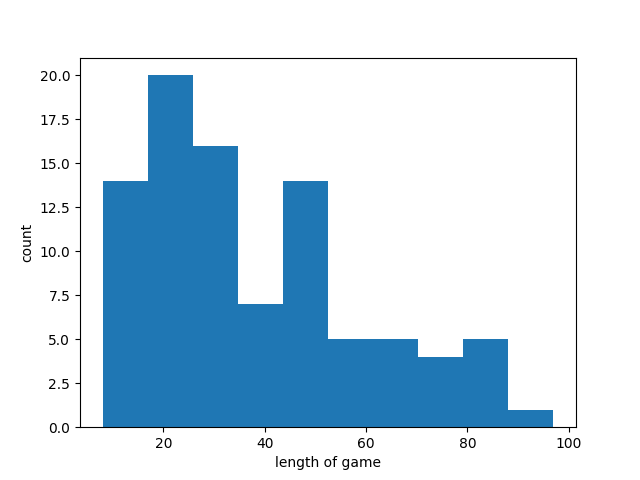
\includegraphics[width=.5\textwidth]{snakes_and_ladders_length_histogram.png}
	\caption{Histogram showing the number of transitions to complete Snakes and Ladders for 100 trials.}
	\label{snakes_and_ladders}
\end{figure}

\paragraph{3.}
We can model the ``frog puzzle'' with $N$ pads as a finite Markov process. The state space $\mathcal{S} = \{s_0,\dots,s_{N}\}$ has an initial state $s_0$ and a terminal state $\mathcal{T} = \{s_{N}\}$. The transition model is, $\mathcal{P}(S_{t+1} = s_{t+i}, \forall i \in [1, N-t] | S_t = s_t) = \frac{1}{N - t}$. This encodes that at each pad, the frog has equal probability of hopping on any of the remaining pads.

The problem is solved numerically for $N = 10$ by generating traces for the Markov process. Fig. \ref{frog_puzzle} shows a histogram with the number of hops used to jump across the river/pond/pads over 10000 trials. See $\texttt{frog.py}$. The mean number of hops of the trials was 2.8132.
\begin{figure}
	\centering
	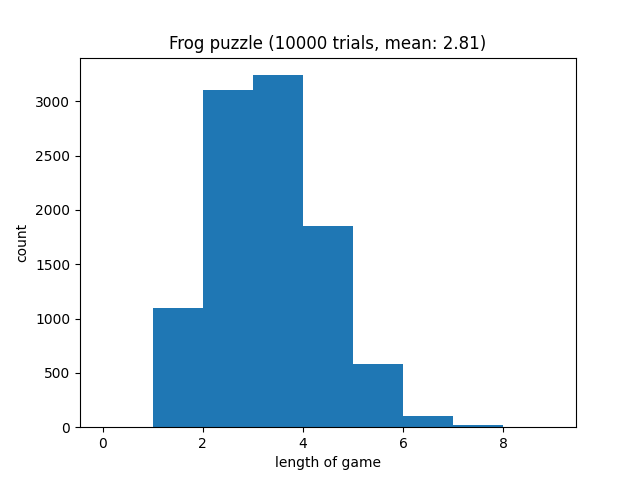
\includegraphics[width=.5\textwidth]{frog_puzzle_histogram.png}
	\caption{Histogram showing the number of transitions to complete ``frog puzzle" for 10000 trials.}
	\label{frog_puzzle}
\end{figure}

\paragraph{4.}
The reward model to compute the expected number of rolls to complete the game should simply be 1 for each transition, undiscounted. Computing the expectation of this reward exact corresponds to computing the expected number of rolls to complete the game. See $\texttt{snakes\_and\_ladders\_mrp.py}$.

\paragraph{5.}
The first stock example has been extended, see \texttt{stonks.py}. The reward for a given stock price can be set by defining the function \texttt{stock_reward}. The cumulative discount reward can then be compute by simulating the MRP for a large number of time steps. The value function for a given initial state can be compute by approximating the expected value function a state using many traces.

\end{document}
